La gràfica de la funció $f$ és la paràbola del dibuix, i $F$ és una primitiva de $f$.
\begin{center}
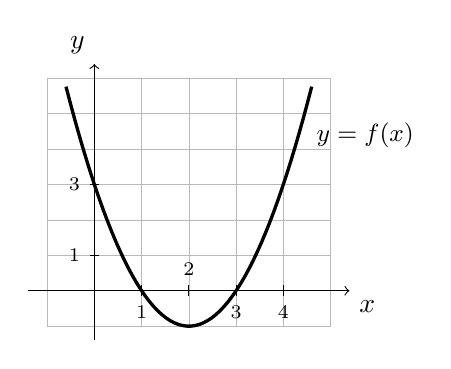
\begin{tikzpicture}[x=0.6cm,y=0.45cm]
  \draw[gray!55,very thin,step=1] (-1,-1) grid (5,6);
  \draw[->] (-1.4,0) -- (5.4,0) node[below right] {$x$};
  \draw[->] (0,-1.4) -- (0,6.4) node[above left] {$y$};
  \foreach \i in {1,3,4} \draw (\i,0.15) -- (\i,-0.15) node[below,font=\scriptsize] {$\i$};
  \draw (2,0.15) -- (2,-0.15) node[pos=0,above,font=\scriptsize] {$2$};
  \foreach \j in {1,3} \draw (0.1,\j) -- (-0.1,\j) node[left,font=\scriptsize] {$\j$};
  \draw[\colorgrafica,very thick,domain=-0.6:4.6,samples=60] plot (\x,{\x*\x-4*\x+3});
  \node[\colorgrafica,font=\small,right] at (4.5,4.4) {$y=f(x)$};
\end{tikzpicture}
\end{center}

\begin{apartats}

\apartat[1,25]{0,75}
Llegint la gràfica de $f$, troba els intervals de creixement i de decreixement de $F$, i les abscisses
dels seus extrems relatius.

\begin{solucio}
Com que $F'(x)=f(x)$ per a tot $x$, $F$ creix on $f>0$ i decreix on $f<0$. La paràbola talla l'eix a
$x=1$ i $x=3$: $F$ creix a $(-\infty,1)$ i a $(3,+\infty)$, i decreix a $(1,3)$. Té un màxim relatiu a
$x=1$ i un mínim relatiu a $x=3$.
\end{solucio}

\begin{tria}{primitiva-grafica}
\itemtria{expressio}{1}{1,25}
Troba l'expressió de $f$ a partir de la gràfica, i la primitiva $F$ que compleix $F(0)=0$. Quant valen
el màxim i el mínim relatius de $F$?

\begin{solucio}
La paràbola té arrels 1 i 3 i passa per $(0,3)$: $f(x)=a(x-1)(x-3)$ amb $3a=3$, és a dir,
$f(x)=x^2-4x+3$. Les primitives són $\frac{x^3}{3}-2x^2+3x+k$, i $F(0)=0$ dona $k=0$.\\
Màxim: $F(1)=\frac13-2+3=\frac43$. Mínim: $F(3)=9-18+9=0$.
\end{solucio}

\itemtria{curvatura}{1}{1,25}
Troba els intervals de concavitat i de convexitat de $F$ i el seu punt d'inflexió. Dibuixa l'aspecte
que té la gràfica d'una primitiva $F$.

\begin{solucio}
$F''(x)=f'(x)$: la curvatura de $F$ la dona el creixement de $f$. La paràbola decreix a $(-\infty,2)$ i
creix a $(2,+\infty)$; per tant, $F''<0$ a $(-\infty,2)$, on $F$ és còncava ($\cap$), i $F''>0$ a
$(2,+\infty)$, on és convexa ($\cup$). El punt d'inflexió és a $x=2$, el vèrtex de la paràbola.\\
La gràfica de $F$ és la d'una cúbica que puja fins al màxim a $x=1$, baixa fins al mínim a $x=3$
canviant de curvatura a $x=2$, i torna a pujar.
\end{solucio}
\end{tria}

\begin{nomesllarg}
\apartat{0,75}
Com és la gràfica de $f'$? Relaciona el seu signe amb el creixement de $f$.

\begin{solucio}
$f'(x)=2x-4$: una recta que talla l'eix a $x=2$. És negativa a $(-\infty,2)$, on la paràbola decreix, i
positiva a $(2,+\infty)$, on creix. Al vèrtex, $f'(2)=0$.
\end{solucio}
\end{nomesllarg}

\end{apartats}
